%!TEX root = ../Dimensionieren I.tex

\chapter{Tabellenwerte für Elementare Beanspruchungen} % (fold)
	\section{Torsion} % (fold)
		\label{torsion}
		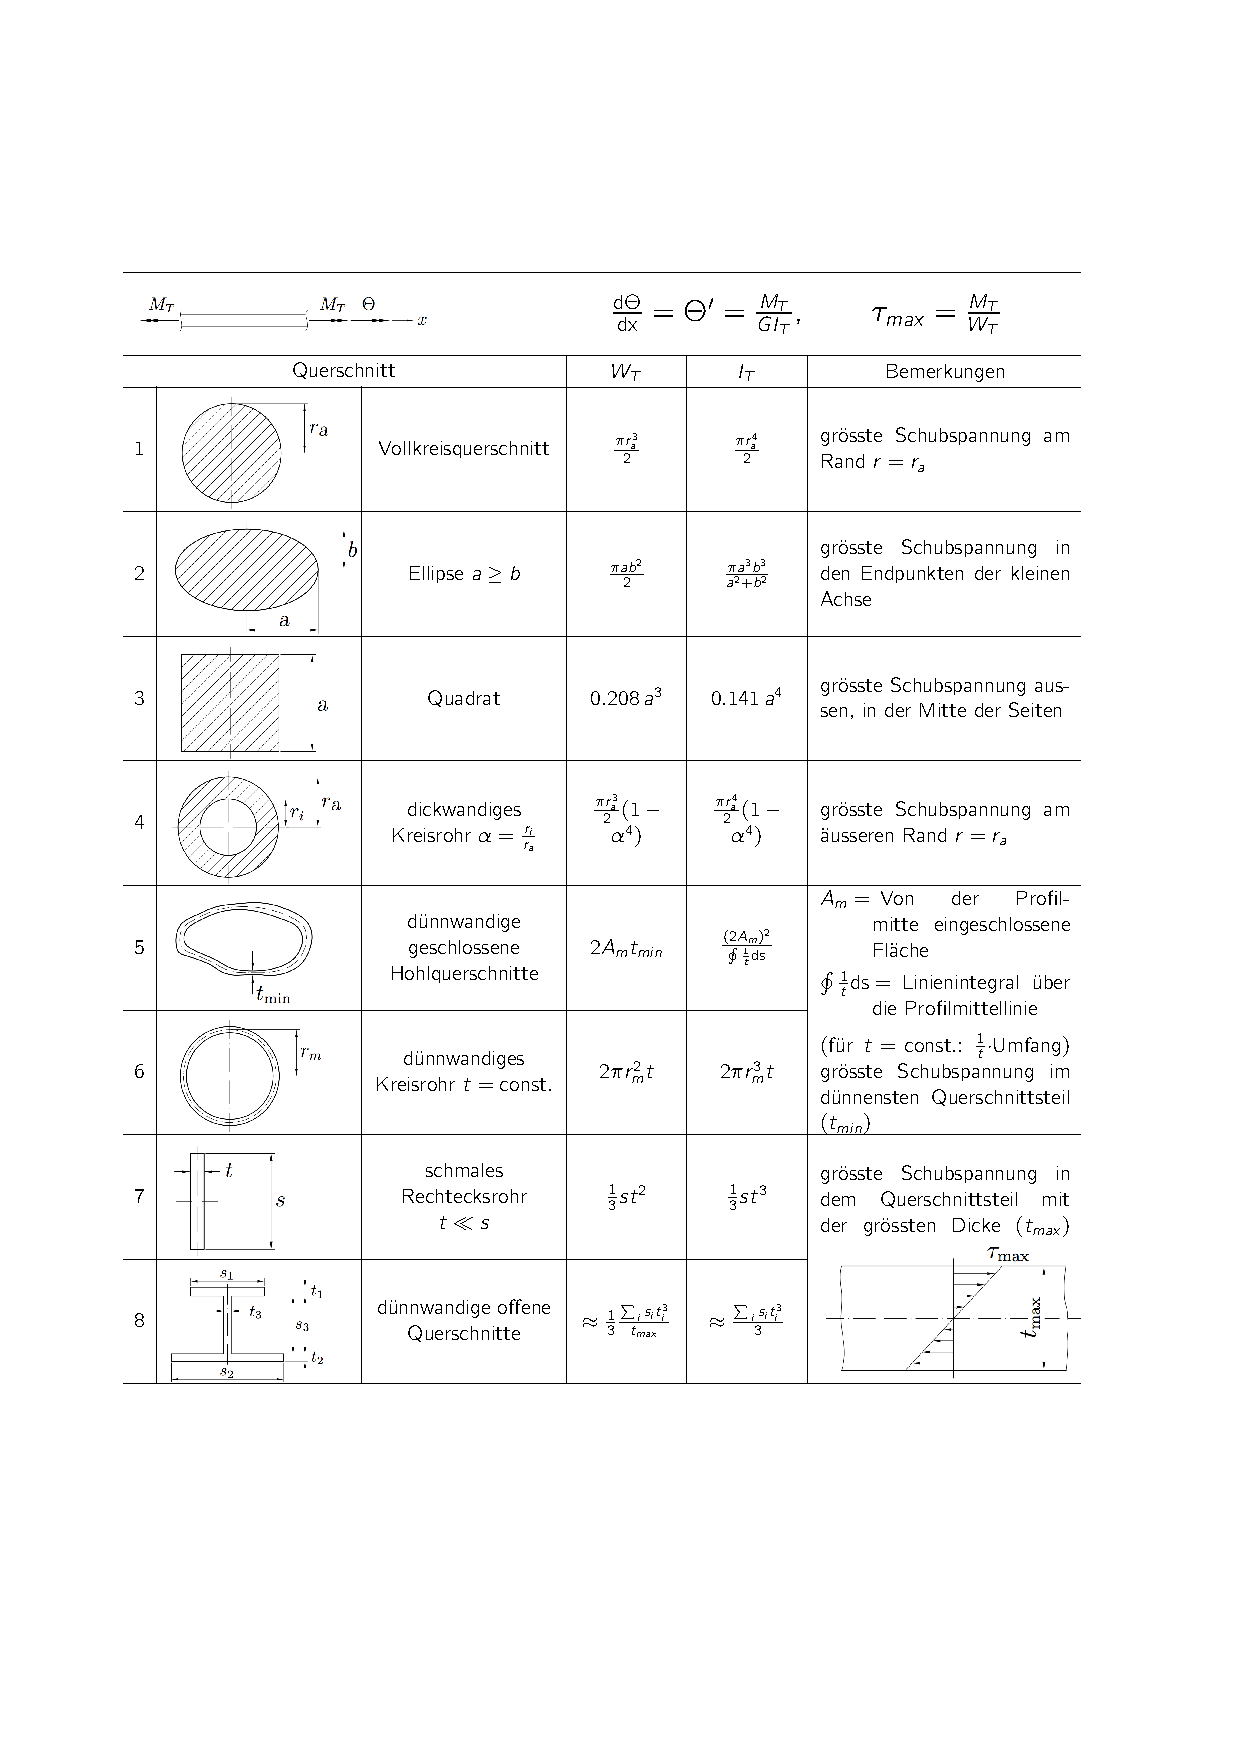
\includegraphics[width=\columnwidth]{graphics/darmstadt}

		\begin{center}
			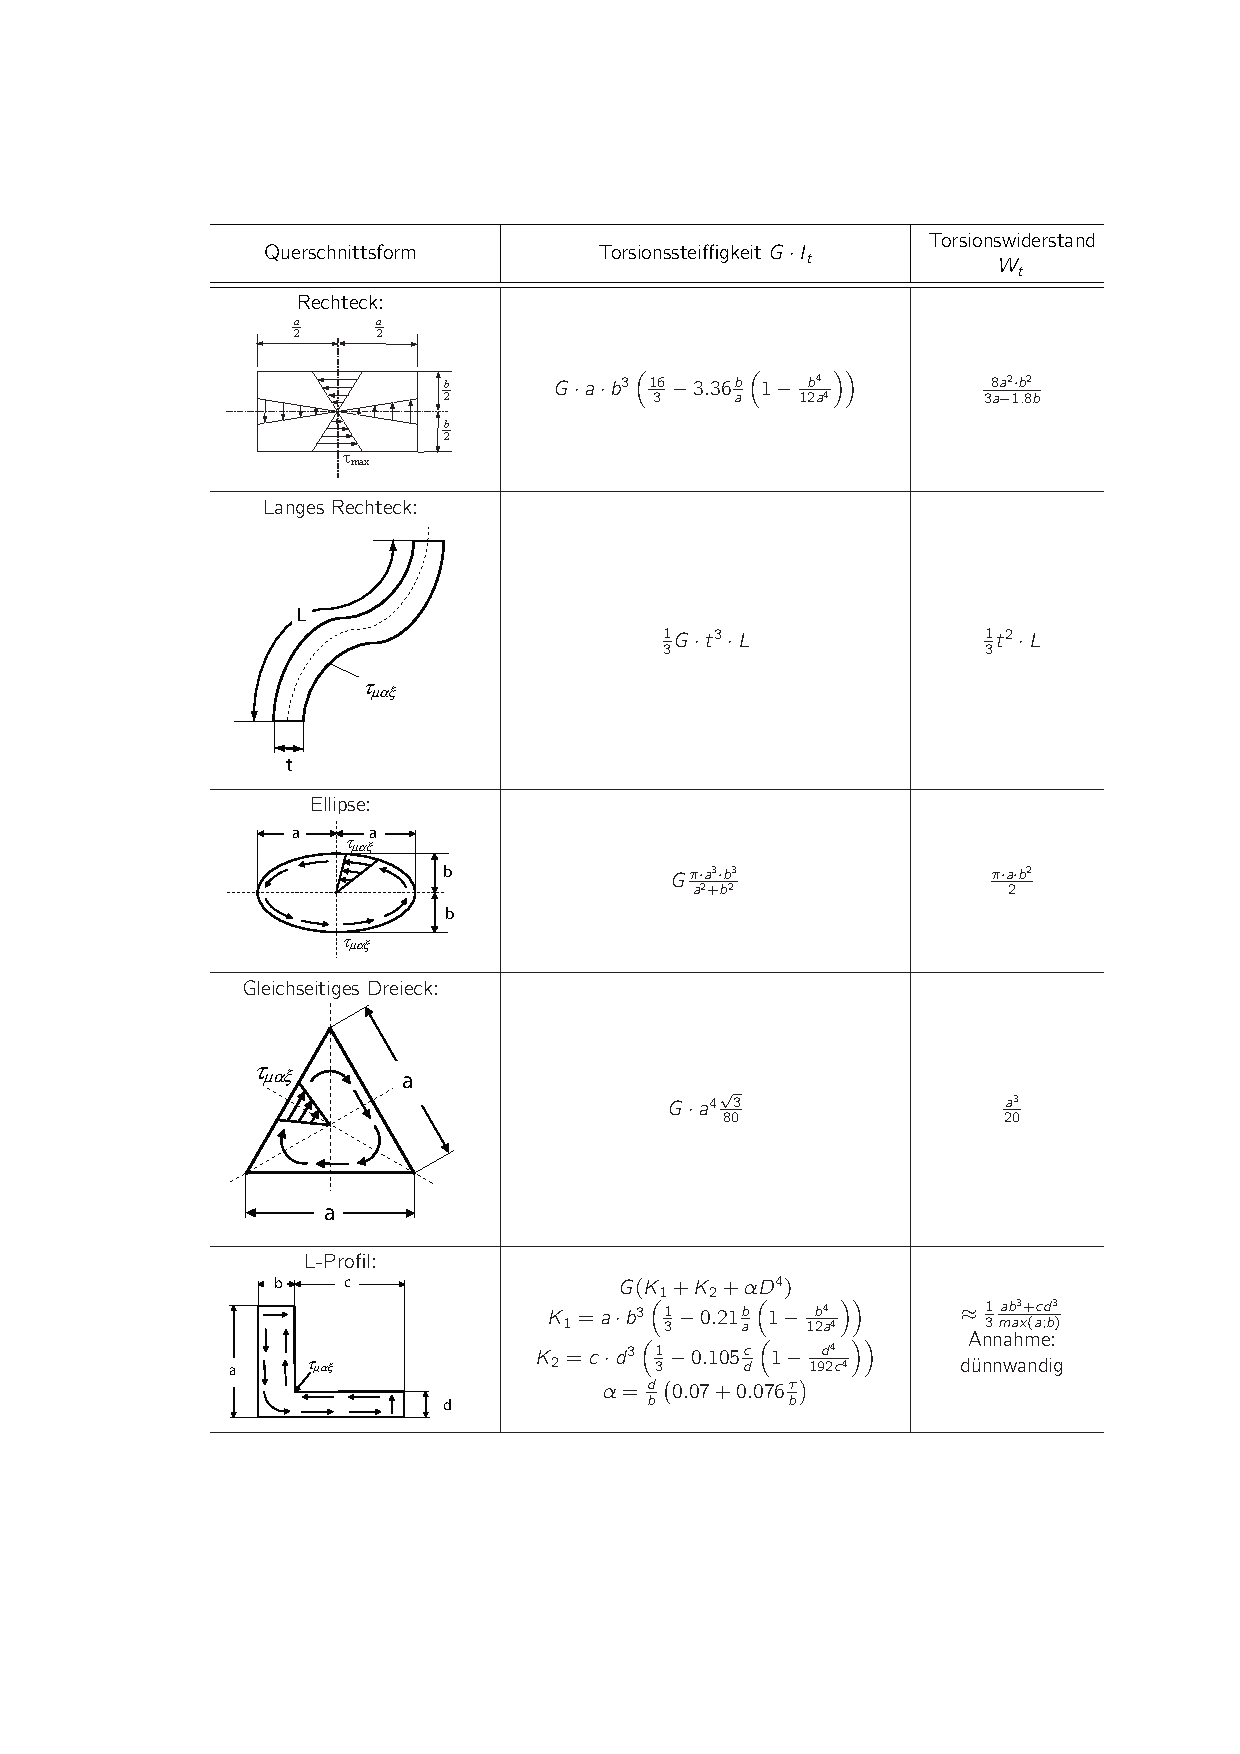
\includegraphics[width=.975\columnwidth]{graphics/torsion}
		\end{center}
	% section: Torsion (end)
\end{multicols}
\begin{multicols}{3}
	\section{Trägheitsmomente} % (fold)
		\begin{center}
			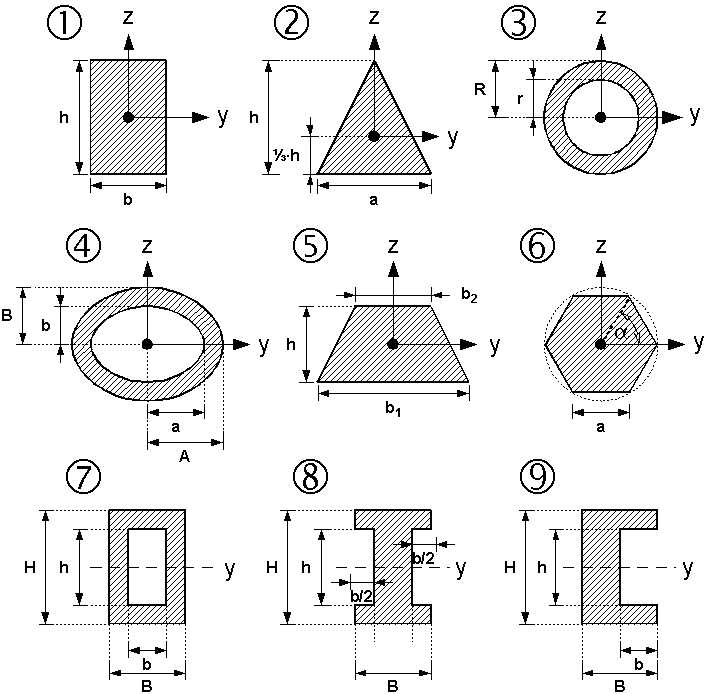
\includegraphics[width=\columnwidth]{graphics/traegheit}
		\end{center}
		
		% \begin{multicols}{2}
		% 	\setlength{\mathindent}{0pt}
			\begin{enumerate}
				\item Rechteck:
					\begin{equation*}
						I_y = \frac{b\cdot h^3}{12}, \quad I_z = \frac{h\cdot b^3}{12}
					\end{equation*}
				\item Dreieck:
					\begin{equation*}
						I_y = \frac{a \cdot h^3}{36}, \quad I_z = \frac{h \cdot a^3}{48}
					\end{equation*}
				\item Kreisring:
					\begin{equation*}
						I_y = I_z = \frac{\pi}{4}\cdot (R^4 - r^4)
					\end{equation*}
				\item Ellipsenring:
					\begin{align*}
						I_y &= \frac{\pi}{4}\cdot (A\cdot B^3 - a \cdot b^3) \\
						I_z &= \frac{\pi}{4}\cdot (A^3\cdot B - a^3 \cdot b)
					\end{align*}
				\item Symmetrisches Trapez:
					\begin{align*}
						I_y &= h^3 \cdot \frac{(b_1 + b_2)^2 + 2 \cdot b_1b_2}{36 \cdot (b_1 + b_2)} \\
						I_z &= \frac{h}{48}\cdot (b_1 + b_2) \cdot (b_1^2 + b_2^2)
					\end{align*}
				\item Regelmässiges n-Eck:
					\begin{equation*}
						I_y = I_z = \frac{n}{96}\cdot a^4 \cdot \frac{2 + \cos(\alpha)}{(1-\cos(\alpha))^2}\cdot \sin(\alpha)
					\end{equation*}
				\item[7. - 9.] Kastenprofil:
					\begin{align*}
						I_y &= \frac{1}{12}\cdot (B\cdot H^3 - b \cdot h^3) \\
						I_z &= \frac{1}{12}\cdot (B^3\cdot H - b^3 \cdot h)
					\end{align*}
			\end{enumerate}
		% \end{multicols}
	% section: Trägheitsmomente (end)
% chapter: Tabellenwerte für Elementare Beanspruchungen (end)
\chapter{Tabellenwerte für Ermüdungsfestigkeit} % (fold)
	\section{Wechselfestigkeit} % (fold)
		\subsection{Allgemeine Baustähle} % (fold)
			\label{baustaehle}
			$d_{\text{B}} \leq 16$ \\
			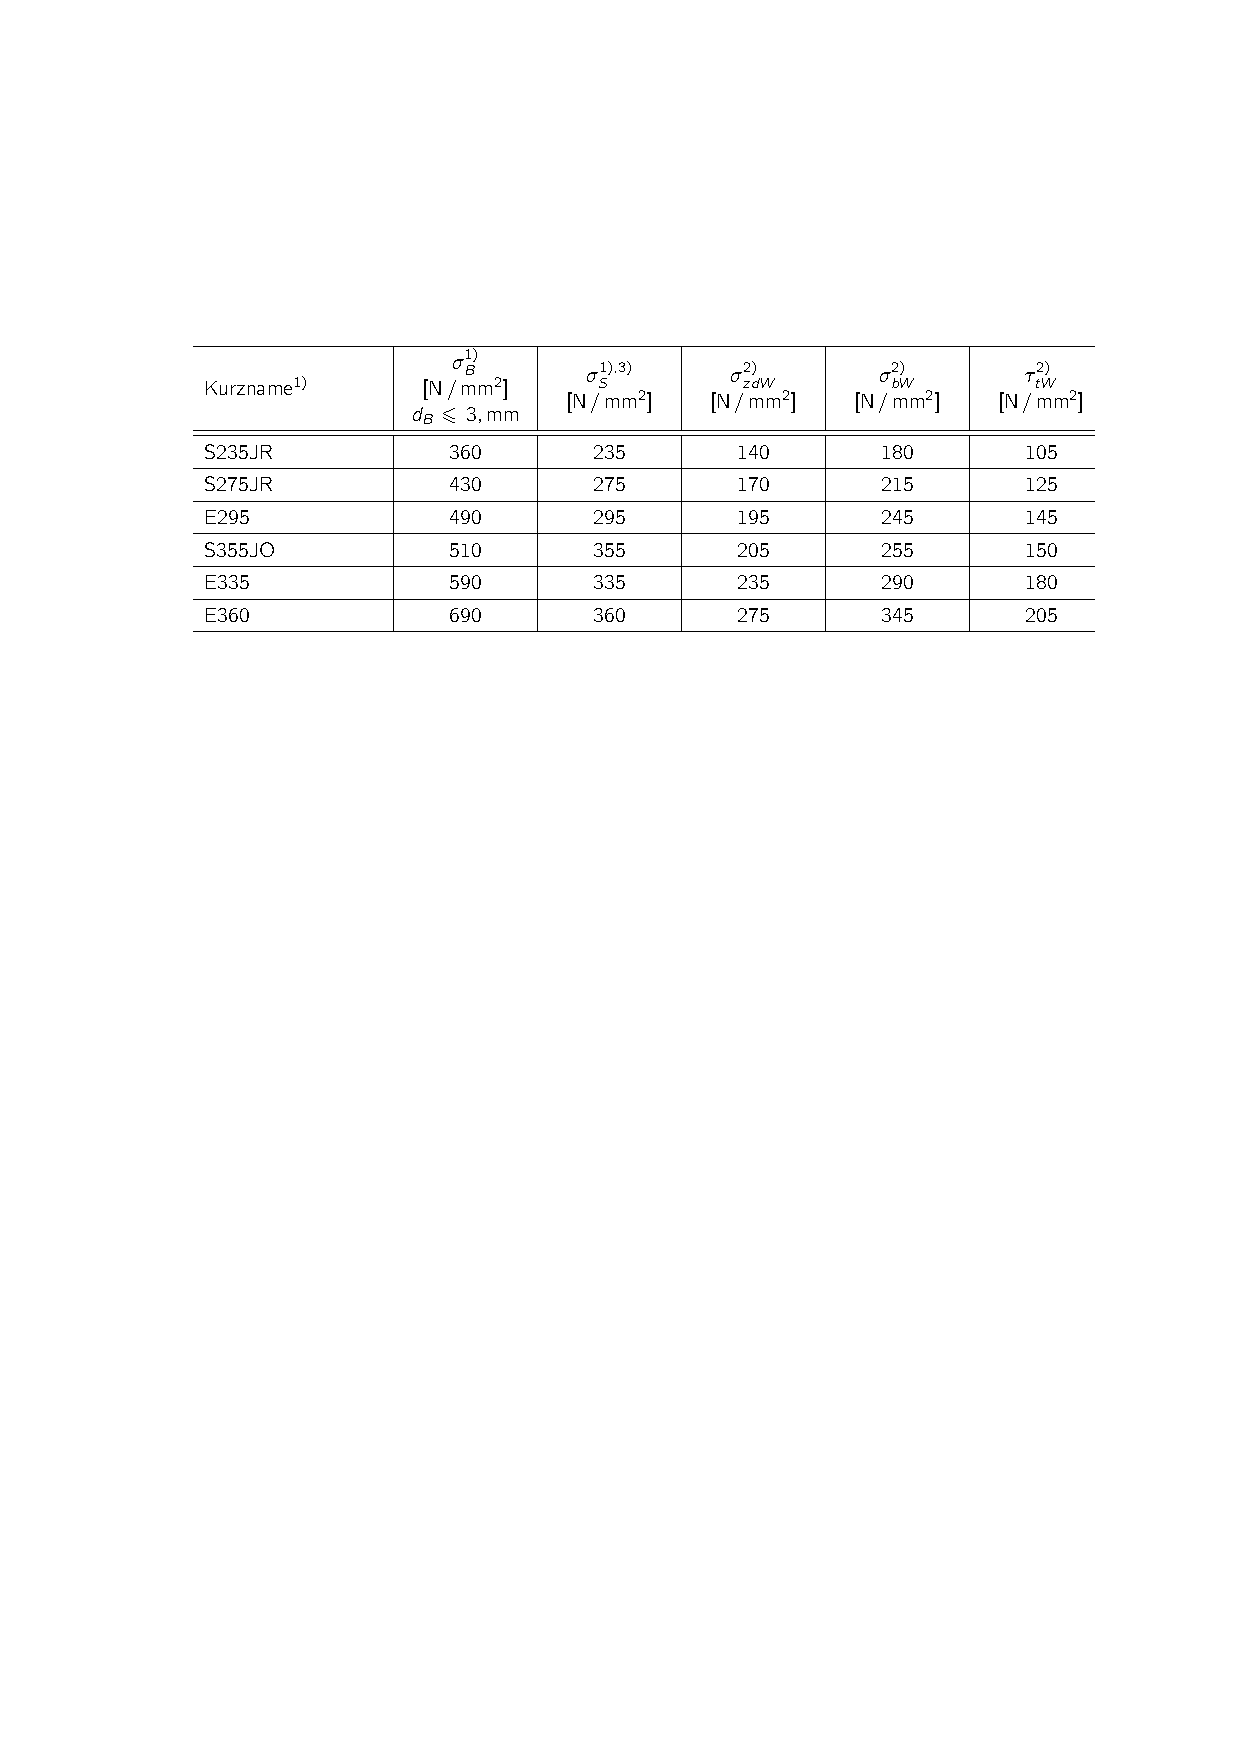
\includegraphics[width=\columnwidth]{graphics/baustaehle}
		% subsection: Allgemeine Baustähle (end)
		\subsection{Einsatzstähle} % (fold)
			\label{einsatzstaehle}
			$d_{\text{B}} \leq 11$ \\
			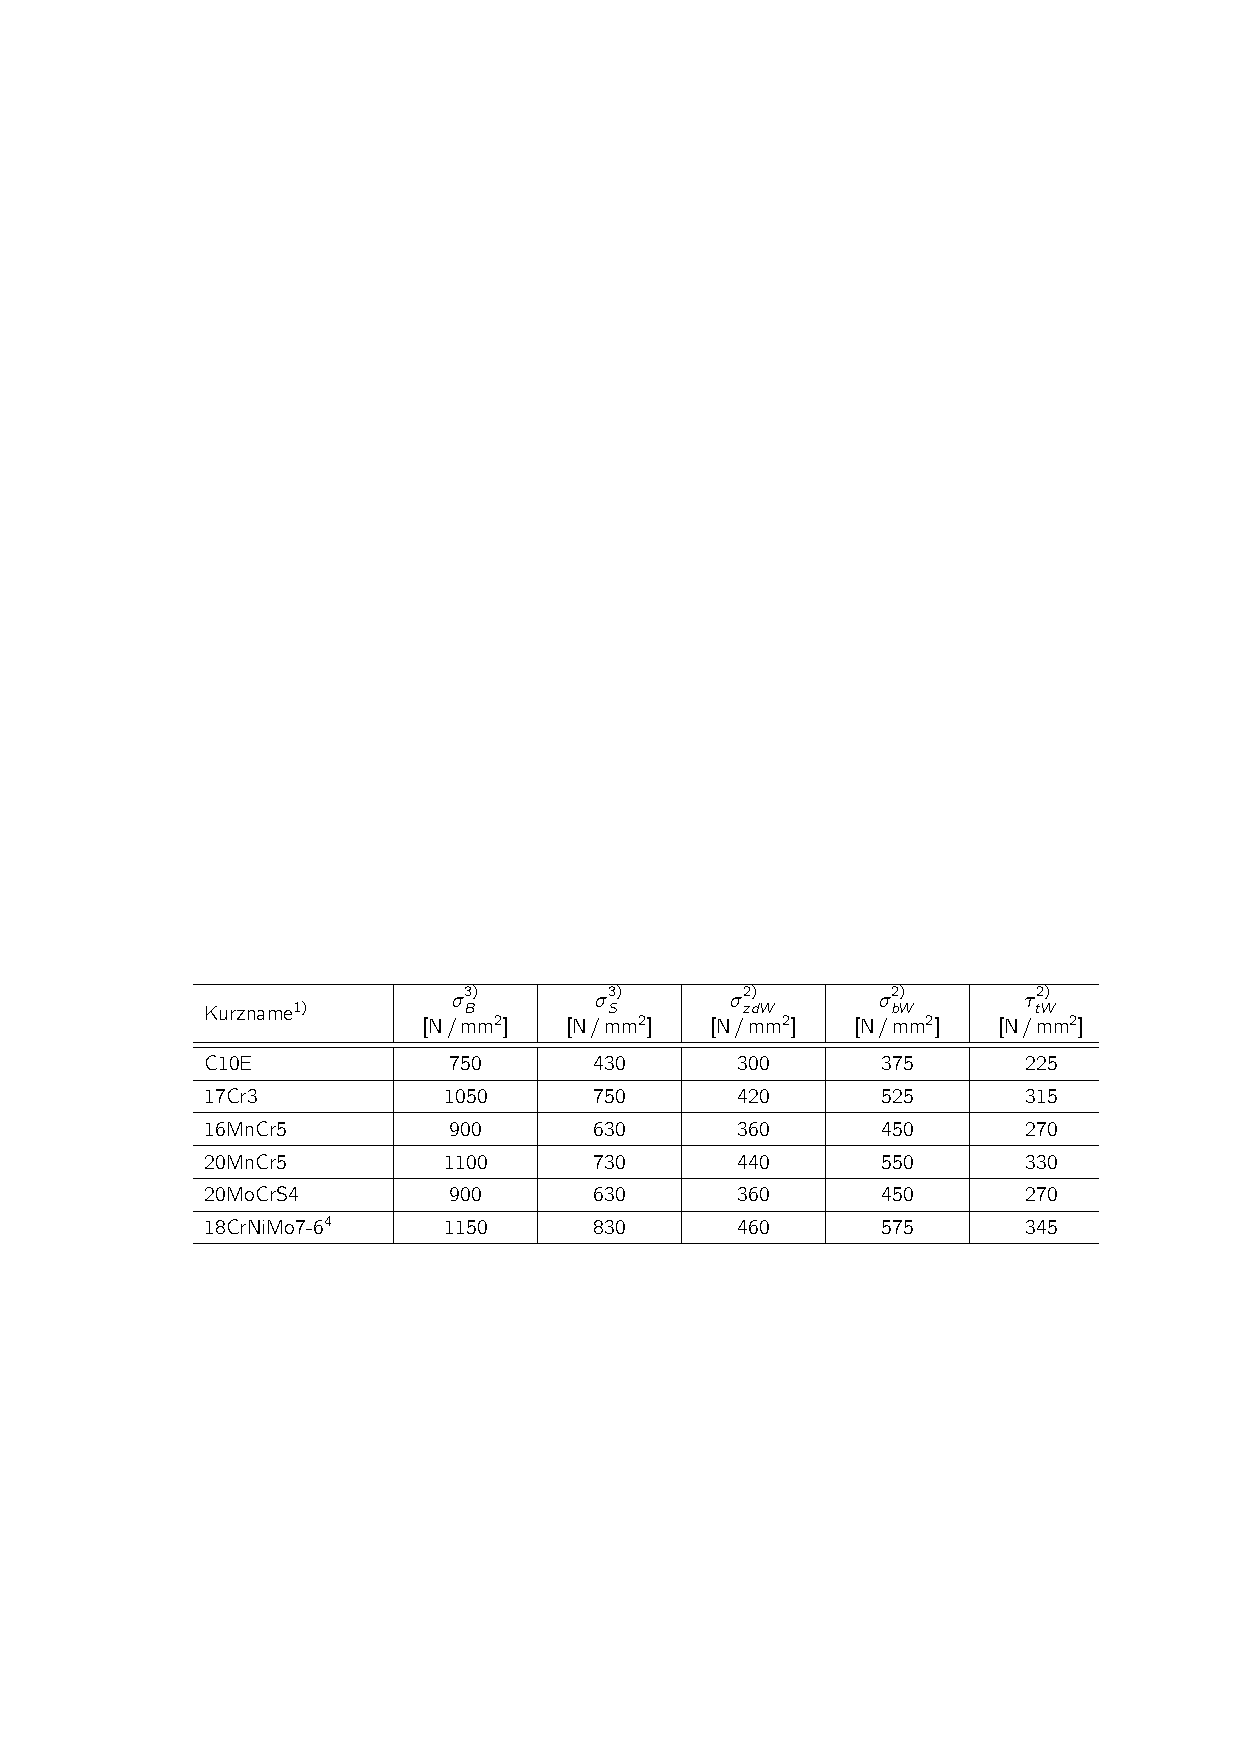
\includegraphics[width=\columnwidth]{graphics/einsatzstaehle}
		% subsection: Einsatzstähle (end)
		\subsection{Vergütungsstähle} % (fold)
			\label{verguetungsstaehle}
			$d_{\text{B}} \leq 16$ \\
			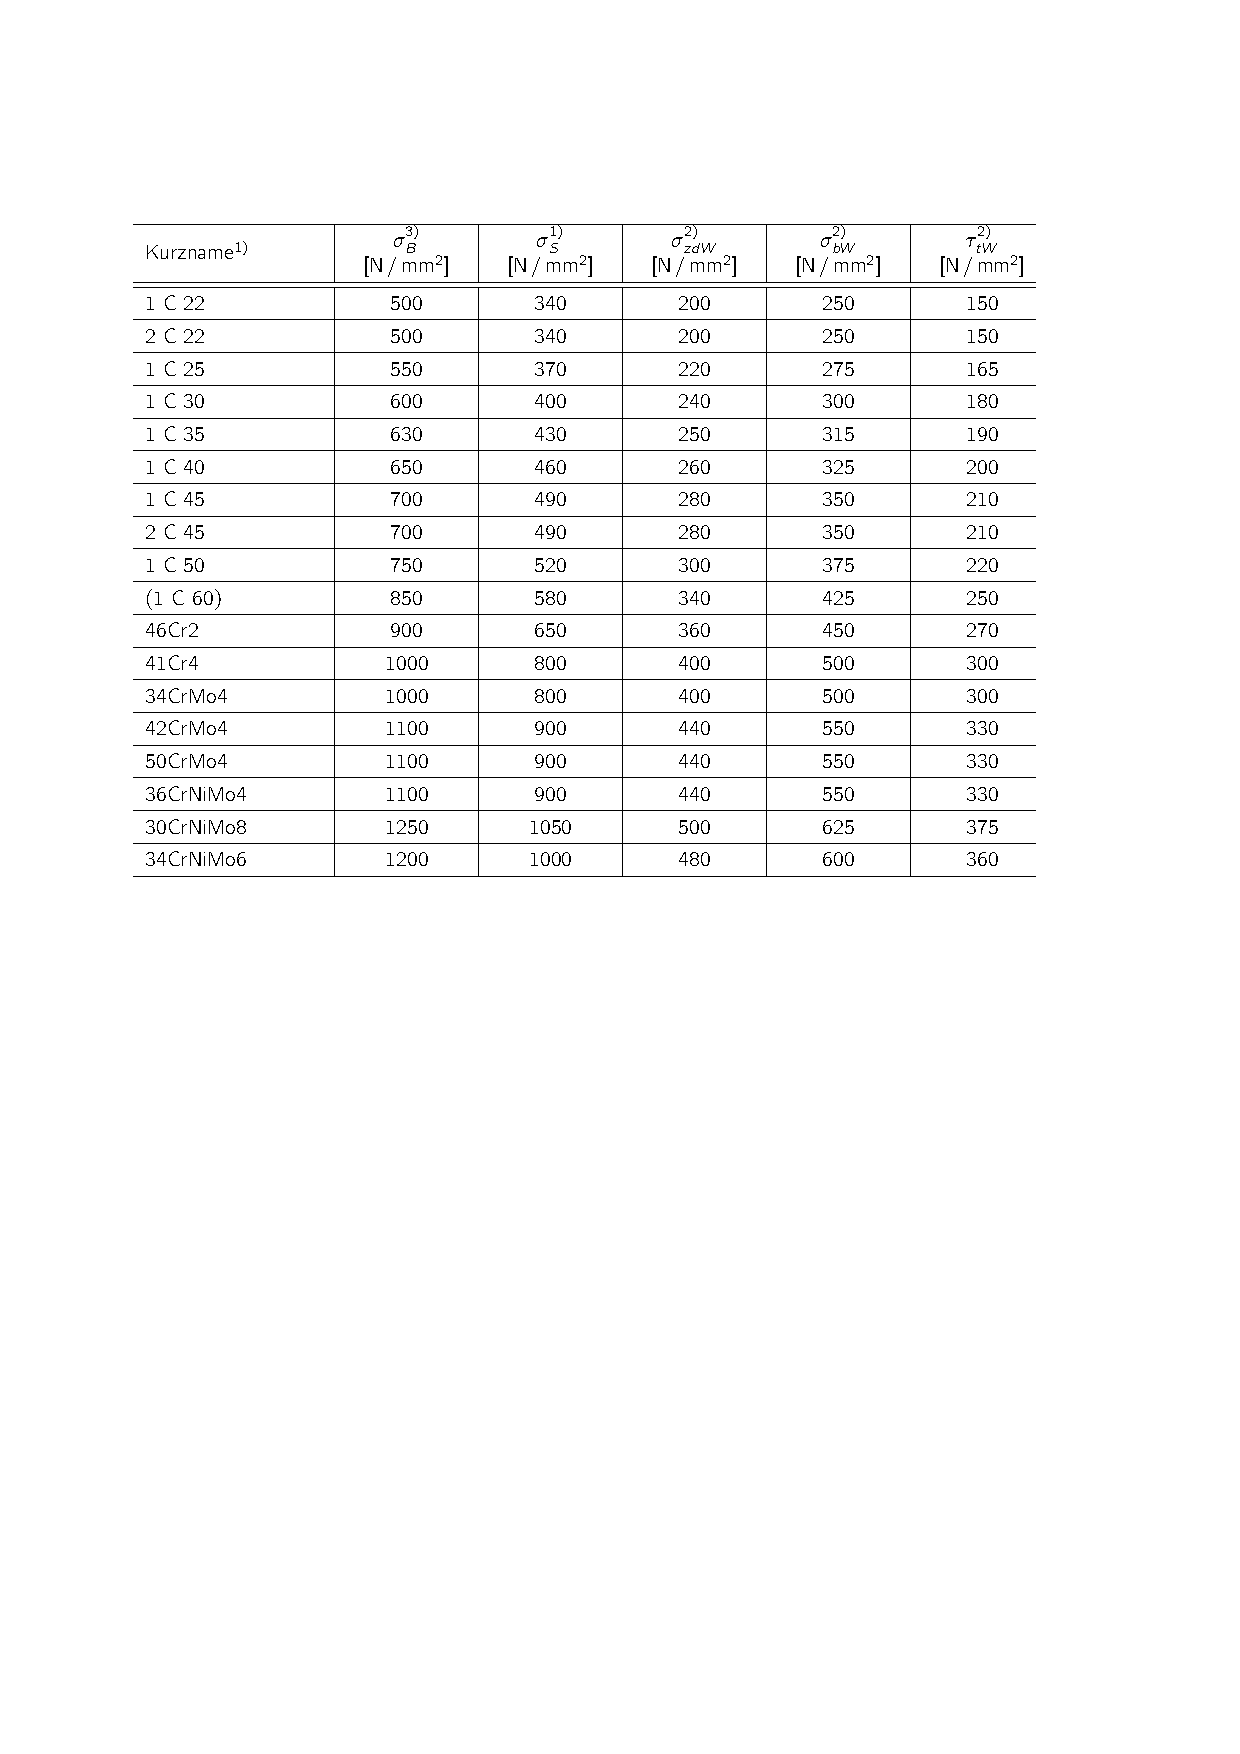
\includegraphics[width=\columnwidth]{graphics/verguetungsstaehle}
		% subsection: Vergütungsstähle (end)
		\subsection{Nitrierstähle} % (fold)
			\label{nitrierstaehle}
			$d_{\text{B}} \leq 100$ \\
			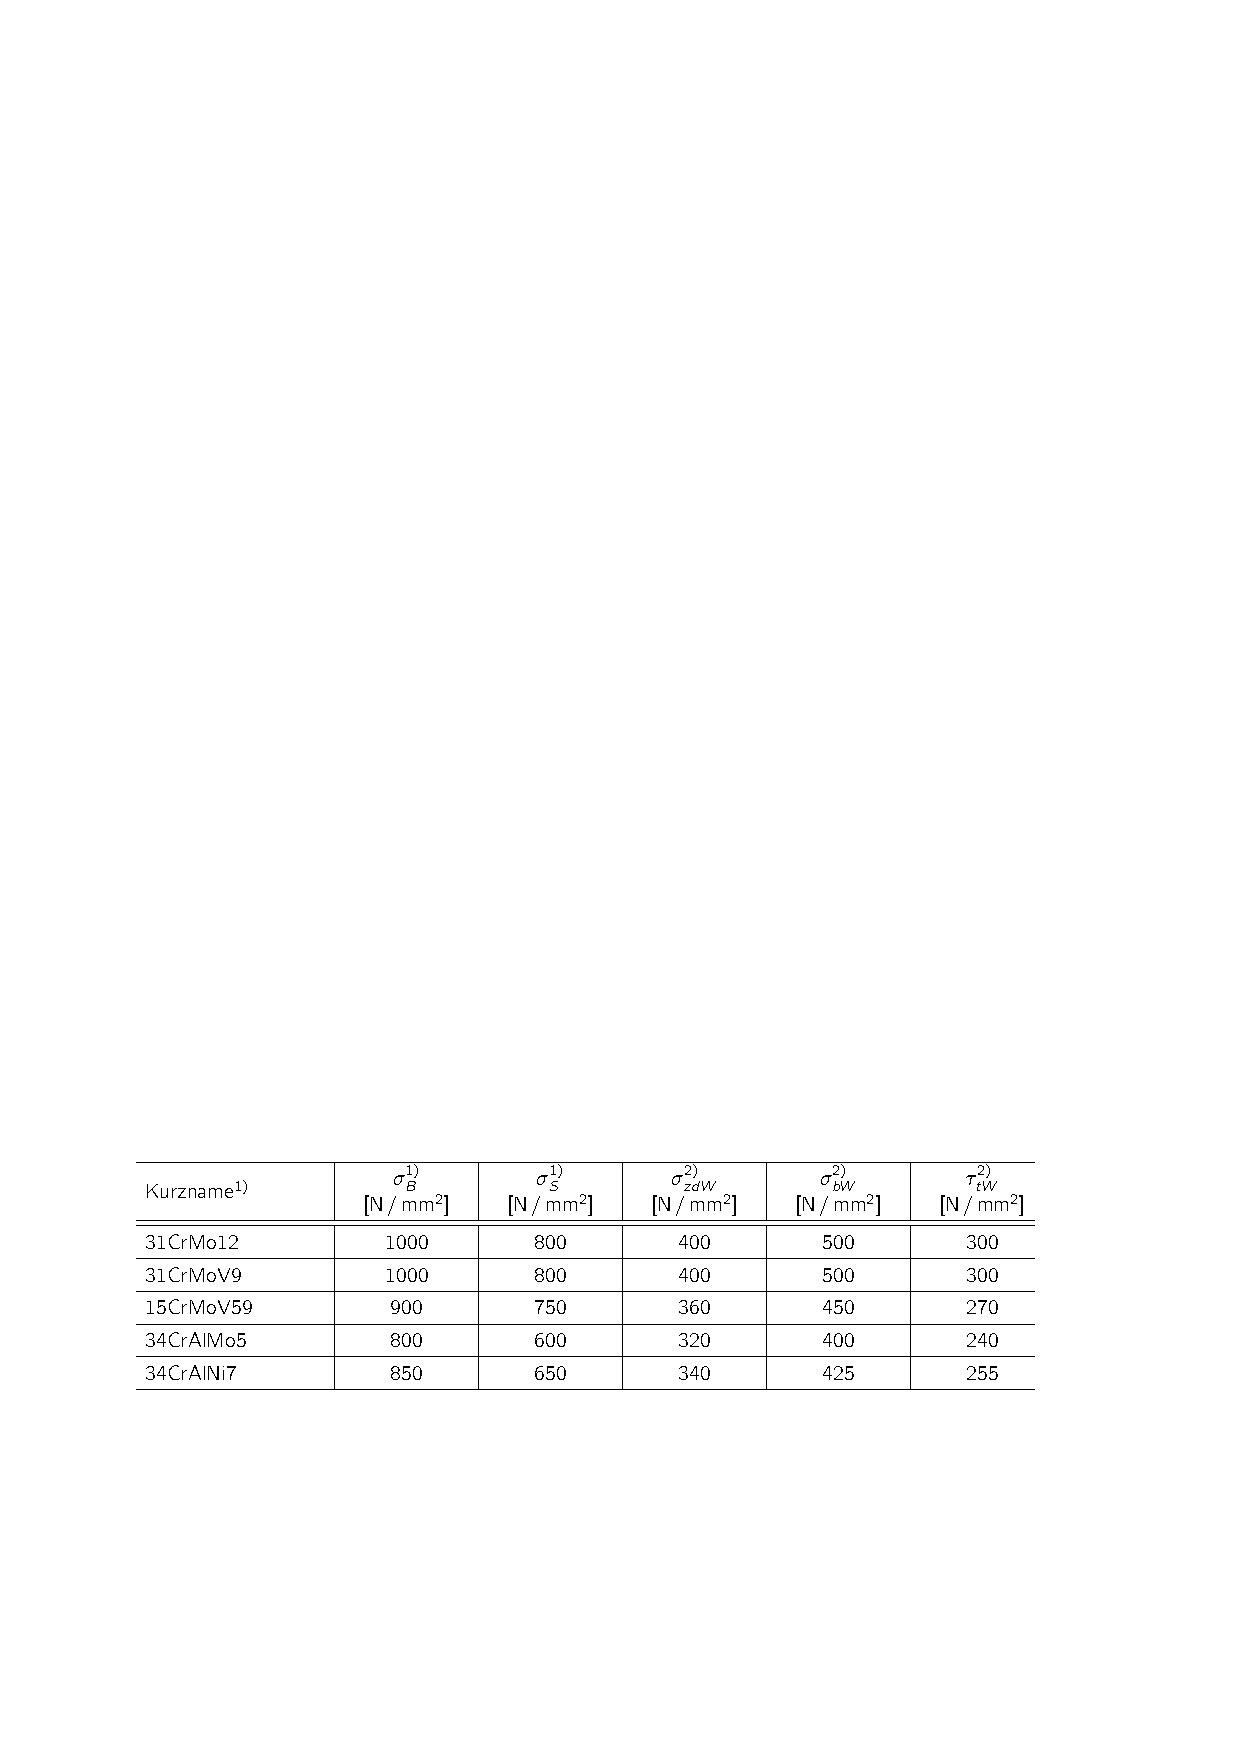
\includegraphics[width=\columnwidth]{graphics/nitrierstaehle}
		% subsection: Nitrierstähle (end)
	% section: Wechselfestigkeit (end)
% chapter: Tabellenwerte für Ermüdungsfestigkeit (end)
\chapter{Tabellenwerte Niet-, Stift- und Bolzenverbindungen} % (fold)
	\label{flaechenbelastungen}
	\section{Zulässige Festigkeitswerte} % (fold)
		Für Stifte und Bolzen:
		\begin{equation*}
			\sigma_{\text{zul}}=\frac{\sigma_{\text{F}}}{S_{\text{F}}} \quad \text{mit } S_{\text{F}}\in [1.5 , 2]
		\end{equation*}
		Für Bohrungen:
		\begin{equation*}
			\text{Ruhende Belastung:} \quad p_{\text{zul}} \leq 0.4 \cdot \sigma_B
		\end{equation*}
		\begin{equation*}
			\text{Schwellende Belastung:} \quad p_{\text{zul}} \leq 0.3 \cdot \sigma_B
		\end{equation*}
		\begin{equation*}
			\text{Wechselnde Belastung:} \quad p_{\text{zul}} \leq 0.2 \cdot \sigma_B
		\end{equation*}
	% section: Zulässige Festigkeitswerte (end)
	\section{Empfohlene Flächenbelastungen drehender Bolzenverbindungen} % (fold)
		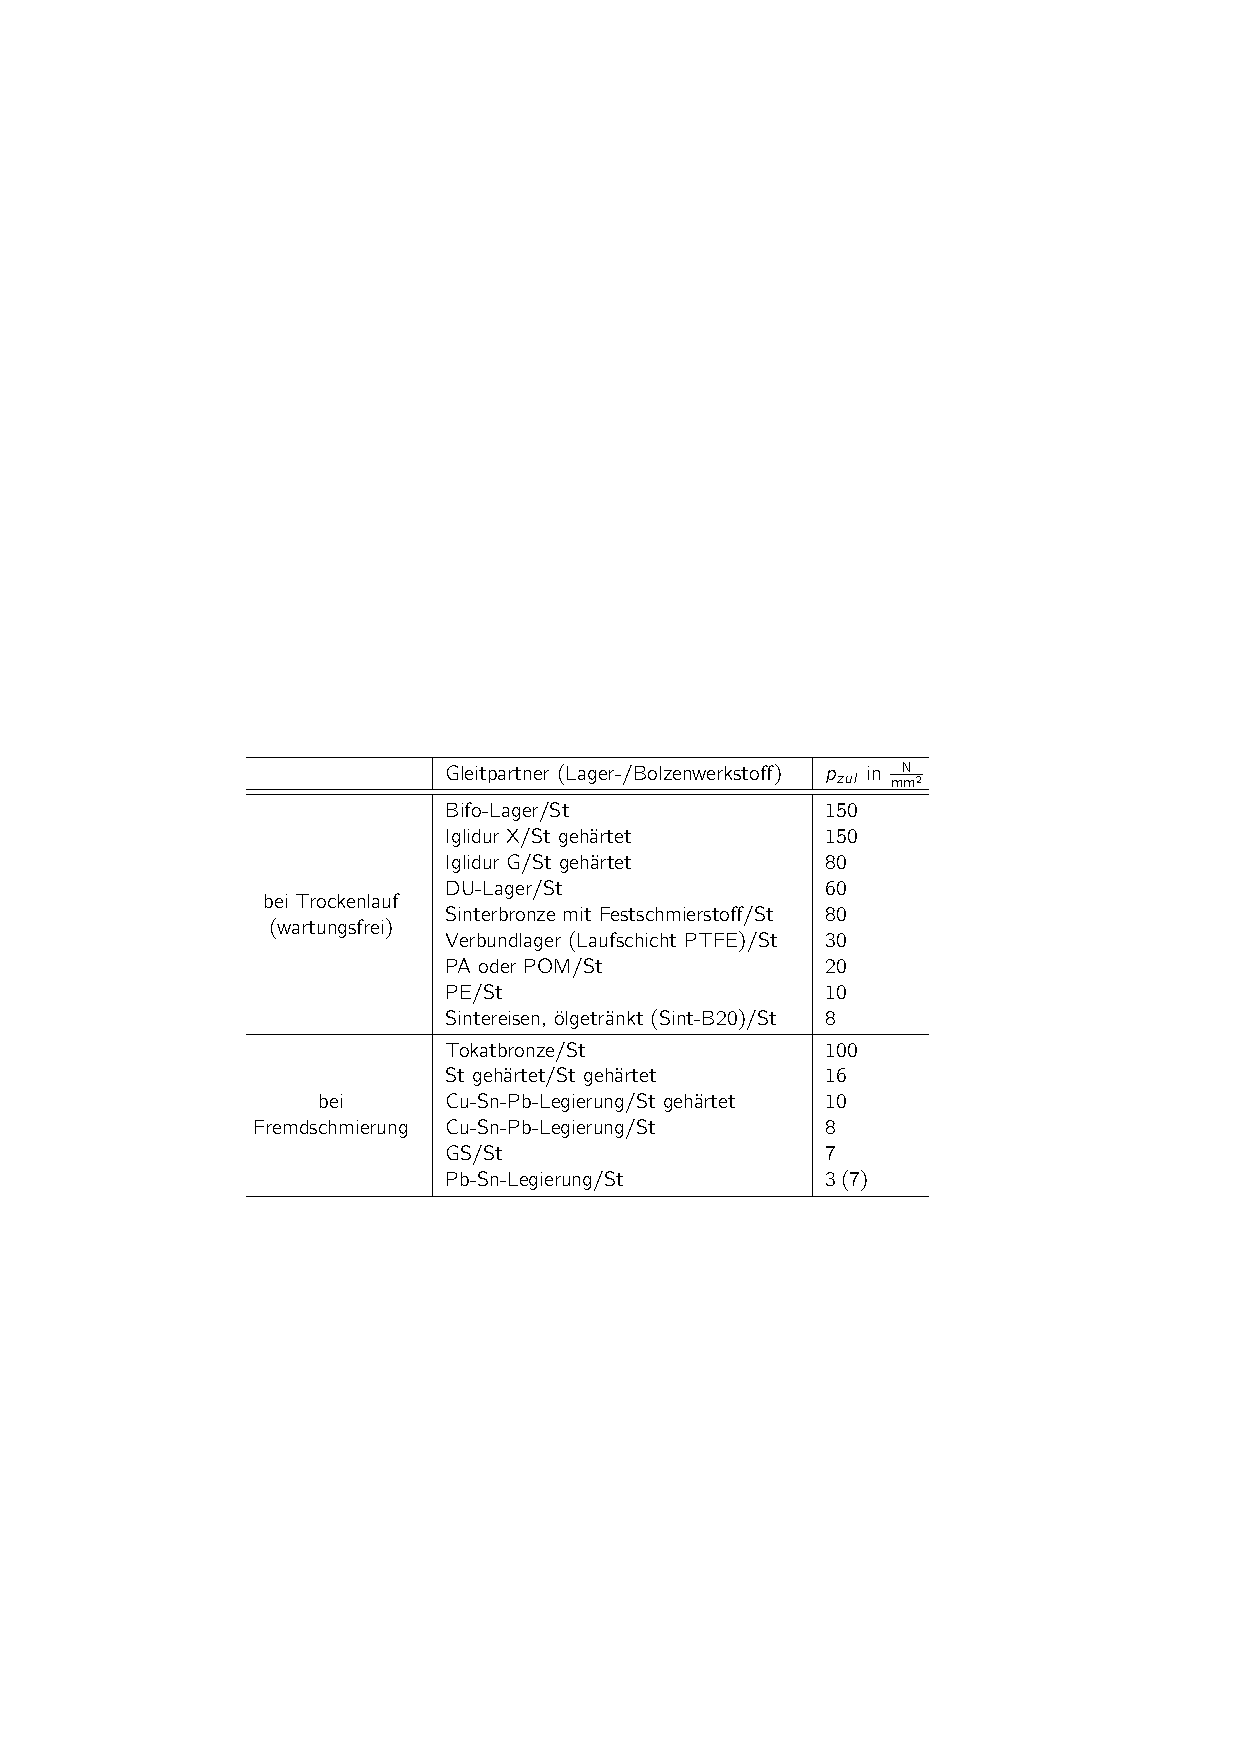
\includegraphics[width=\columnwidth]{graphics/flaechenbelastungen}
	% section: Empfohlene Flächenbelastungen drehender Bolzenverbindungen (end)
% chapter: Tabellenwerte Niet-, Stift- und Bolzenverbindungen (end)